%% ===================================================================
\section{Results}
\label{sec:results}
%% ===================================================================

\subsection{Architecture Choice Reverses Recovery Across Targets}
\label{sec:results-interaction}

Since Eq.\,6 and V16 use different native initialization
protocols (Section~\ref{sec:setup}), recovery-rate comparisons
are best read as architecture-plus-native-training-protocol
comparisons unless otherwise noted.  The results below separate
three questions: whether architecture changes recovery, whether
the effect persists across operator asymmetry, and whether
held-out validation can reduce architecture-specific failures.
Fig.~\ref{fig:heatmap} shows that recovery cannot be attributed
to just architecture or target.  Recovery is governed by the
specific architecture--target pairing.
Eq.\,6 acts as a specialist with 100\% recovery on two targets, 0\% on
three, and below 2\% on the remaining one.  V16 recovers all four
chain targets at rates between 16\% and 99.6\%, with $x \leftrightarrow
y$ symmetry inherited from its leaf-only variable design.  Hybrid is
an RL specialist, recovering 95--96\% on RL targets and near 0\%
elsewhere.  No single architecture dominates.  Eq.\,6 reaches 100\%
where V16 reaches 17\%, yet V16 reaches 99.6\% where Eq.\,6 reaches
0\%.

In these tested cells, the reversals cannot be explained by
representability.
Eq.\,6's representable set is a strict superset of V16's (every
internal node in Eq.\,6 offers $\{1,x,f_{\text{child}}\} \supset
\{1,f_{\text{child}}\}$, so every V16 tree is also an Eq.\,6
tree), yet Eq.\,6 fails on targets V16 recovers nearly
deterministically.  The failure is therefore not that the
expression is unavailable to the architecture.  The training and
hardening process does not reliably reach the representable
target expression.  Eq.\,6 routes
$x$ through every internal node, so LR targets, whose active
subtree sits on the exponentially amplified left input, receive
strong $x$-gradients early in training, while RL targets place the
active subtree on the attenuated right input and starve $x$ of
signal along the path that must be learned.  Here, starvation
refers to persistently lower gradient norm on the variable path
needed to recover the target.  V16 may avoid this
failure mode because $x$ and $y$ enter only at the leaves through a
shared softmax.  Eq.\,6 nonetheless reaches 100\% on the RR target
with leaves $(y,x)$ despite right-side routing at both levels.
This indicates that leaf assignment interacts with routing
pattern, and that a full account of which combinations succeed
remains open.  Section~\ref{sec:results-gradient}
quantifies the routing imbalance through gradient ratios.

Tracing where each run fails locates the bottleneck.  Across
5{,}376 runs aggregated over initialization strategies, 77\%
reach soft-phase loss below $0.01$, but only 32\% survive the
one-hot snap into a hardened expression with training MSE below
$0.01$, and every one of those then meets the stricter exact-match
tolerances.  The one-hot snap, rather than the final tolerance
threshold, is the main gate.  Failure modes separate by cell.  Eq.\,6/RL under EML
fails during search (soft loss never $<0.01$).  Eq.\,6/RR under
EML reaches a soft fit, but hardening destroys that fit.  EML balanced
cells diverge to $10^{16}$ during search.  SML balanced cells
usually fail during hardening through chain collapse or
snap-induced mismatch.

\subsection{Operator Swap Reverses Shape Preferences}
\label{sec:results-operators}

The asymmetry-direction hypothesis predicts that operators
sharing EML's left-amplification should preserve some
architecture--shape preferences, while reversing the asymmetry
should change those preferences.  Switching from EML to SML
(Fig.~\ref{fig:heatmap}) changes Eq.\,6's preferred shapes,
most clearly on LR and RL.  The LR rate drops from 100\% to 0\%
and the 100\% targets shift to RL$(xy)$ and both RR variants
(Fisher exact $p < 10^{-15}$).  RR remains leaf-assignment
dependent rather than uniformly easy or difficult.  At least one
RR leaf assignment reaches 100\% for Eq.\,6 under both
operators, but the other scores 0\% under EML
(Fig.~\ref{fig:heatmap}).  Since both operators amplify the
left input, the change on LR and RL is consistent with
differences in right-side attenuation ($-1/(1+b^2)$ for SML
versus $-1/b$ for EML).  The
same per-architecture pattern holds across the swap.  Eq.\,6
remains a specialist, V16 recovers 83--100\% on all chains, and
Hybrid remains an RL specialist.

Under EML the right gradient $-1/b$ on $[1,3]$ is moderately
attenuating, enough for V16's symmetric routing to recover RL
targets but not for Eq.\,6's $x$-dominant path.  Under SML the right
gradient $-1/(1+b^2)$ saturates more severely while the left
amplification weakens from $e^a$ to $\cosh a$; the net effect
appears to shift which shapes give Eq.\,6 a favorable balance of gradient
signal between $x$ and $y$ leaves (quantified in
Section~\ref{sec:results-gradient}).  V16's robustness to the
swap is consistent with its leaf-only routing, which does not
commit either variable to a fixed depth.

\begin{figure}[t]
\centering
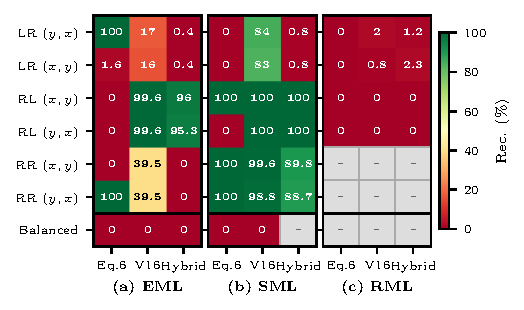
\includegraphics[width=\columnwidth]{fig_odrzywolek2026_heatmap.pdf}
\Description{Heatmap showing recovery rates for three operators across architectures and tree shapes.}
\caption{Exact recovery after hardening depends on the
architecture--target pairing rather than on architecture or
target alone.  Rows are target shapes and leaf assignments;
columns are architectures; panels are operators (EML, SML, RML).
Gray cells: configurations not tested.}
\label{fig:heatmap}
\end{figure}

V16 dominates under SML, recovering all chain targets at 83\% or
above.  Replacing EML with the right-amplified RML collapses
recovery across the board (Eq.\,6: 0\% on every target; V16: 2.0\%
best, $5/256$, 95\% CI $[0.6, 4.5]\%$; Hybrid: RL preference
gone), supporting the interpretation that gradient direction,
rather than operator identity, contributes to the routing
bias.


\subsection{Balanced Trees Resist Recovery Across All Tested Configurations}
\label{sec:results-balanced}

Balanced topologies fail in all tested configurations
($0/3{,}776$; Clopper--Pearson 95\% upper bound $0.10\%$), even
when the same architecture--operator pair recovers chain targets
at high rates.  The failure persists across six training
configurations varying learning rate, iteration budget, and
temperature ($0/192$).  Failure modes differ by operator.  EML
balanced cells diverge during search (loss reaches $10^{16}$),
whereas SML balanced cells often reach a soft fit but collapse
during hardening (44\% chain collapse, 55\% hardening proper).
This suggests that balanced failure is a training-and-hardening
pathology rather than a simple absence of representability.  Branch-wise
gradient measurements in Section~\ref{sec:results-gradient} show
balanced cells with $\rho_{LR}\approx 2$--$3$, several-fold
weaker than the $10$--$17\times$ asymmetry observed on recovered
chains.  This suggests that neither branch receives the
concentrated signal observed in successful chain recoveries.


\subsection{Gradient Asymmetry Correlates with Recovery}
\label{sec:results-gradient}

Two gradient ratios summarize the asymmetry.  The variable-wise
ratio
\begin{equation}
  \rho_{xy}(t) \;=\; \frac{\|\nabla_{\theta_x} \mathcal{L}_t\|}{\|\nabla_{\theta_y} \mathcal{L}_t\|}
  \label{eq:rho-xy}
\end{equation}
compares signal strength on the two variable leaves, and the
branch-wise ratio
$\rho_{LR}(t) = \|\nabla_{\theta_{\text{left}}} \mathcal{L}_t\| \,/\,
\|\nabla_{\theta_{\text{right}}} \mathcal{L}_t\|$
compares signal on the two children of an internal node.  Both are
measured at iteration~1000 across 10 seeds and reported jointly in
Table~\ref{tab:gradients}.  Gradient measurements are reported for the
two most extreme Eq.\,6 targets per operator (100\% and 0\%); the
intermediate targets (T4, T8) are omitted because their mixed
recovery depending on leaf assignment makes the association
ambiguous.  For Eq.\,6 under EML, $\rho_{xy}$ tracks the two
extreme outcomes: $\rho_{xy} < 1$ appears on the 100\% target,
while $\rho_{xy} > 1$ appears on the 0\% target.  Under SML the
correspondence is more nuanced (EML LR: $0.67 \to 100\%$; SML LR:
$1.78 \to 0\%$; SML RL: $1.19 \to 100\%$): the relevant variable
depends on the operator--shape combination, not a universal
threshold.  V16 tolerates a $2.3\times$ imbalance on a 99.6\%
target, suggesting its symmetric leaf-routing provides alternative
pathways that compensate for ratio skew.

\begin{table}[t]
\centering
\caption{Gradient diagnostics at iteration~1000 (10-seed mean
$\pm$ s.e.).  Leaf $\rho_{xy}$ is the variable-wise ratio at
the leaves; branch $\rho_{LR}$ is the left/right gradient-norm
ratio at the root (V16).}
\label{tab:gradients}
\footnotesize
\begin{tabular}{@{}lllrc@{}}
\toprule
Diagnostic        & Arch.\,/Op.\ & Target     & Ratio          & Rec.\ \\
\midrule
Leaf $\rho_{xy}$  & Eq.\,6 EML  & LR\,(yx)  & $0.67\pm0.03$  & 100\% \\
Leaf $\rho_{xy}$  & Eq.\,6 EML  & RL\,(xy)  & $1.58\pm0.04$  & 0\% \\
Leaf $\rho_{xy}$  & Eq.\,6 SML  & LR\,(yx)  & $1.78\pm0.12$  & 0\% \\
Leaf $\rho_{xy}$  & Eq.\,6 SML  & RL\,(xy)  & $1.19\pm0.11$  & 100\% \\
Leaf $\rho_{xy}$  & V16 EML     & RL\,(xy)  & $2.31\pm0.24$  & 99.6\% \\
\midrule
Branch $\rho_{LR}$ & V16 EML    & LR\,(yx)  & $1.20\pm0.06$  & 16.8\% \\
Branch $\rho_{LR}$ & V16 EML    & RL\,(xy)  & $0.06\pm0.01$  & 99.6\% \\
Branch $\rho_{LR}$ & V16 SML    & LR\,(yx)  & $10.0\pm1.2$   & 84.4\% \\
Branch $\rho_{LR}$ & V16 SML    & RL\,(xy)  & $0.07\pm0.00$  & 100\% \\
Branch $\rho_{LR}$ & V16 EML    & Bal\,(xy) & $3.23\pm0.29$  & 0\% \\
Branch $\rho_{LR}$ & V16 SML    & Bal\,(xy) & $2.62\pm0.70$  & 0\% \\
\bottomrule
\end{tabular}
\end{table}

The gradient trajectory (Fig.~\ref{fig:gradient}) shows the
pattern more clearly.  On the 100\% EML target $\rho_{xy}$ briefly
reverses, falling from $1.45$ at iteration~100 to $0.14$ at
iteration~500 before settling at $0.67$ by iteration~1000, and this
$y$-dominated window correlates with convergence.  On the 0\% target
$\rho_{xy}$ stays above $1.14$ throughout.  The trajectory provides
a gradient-level correlate of the architecture--target interaction.
Whether this gradient-level correlate is causal or consequential
is left to Section~\ref{sec:limitations}.

Across the measured configurations, recovery aligns more with the
distribution of gradient signal during training than with any
fixed threshold on $\rho_{xy}$.  V16 recovers when $\rho_{xy}$ sits
near unity, indicating balanced access to both leaves.  Eq.\,6 fails
on RL/EML where $\rho_{xy}$ stays at $1.58$, indicating $y$
starvation.  The same architecture recovers on LR/EML where
$\rho_{xy}$ briefly dips to $0.14$, well below unity, opening a
window in which $y$ can compete.  An operator swap that flips the gradient asymmetry
flips $\rho_{xy}$ and the recovered shape together.  Balanced trees
fit the same picture.  Their branch-wise ratio sits at $\rho_{LR}
\approx 2$--$3$ (Table~\ref{tab:gradients}), several-fold weaker than
the $10$--$17\times$ asymmetry seen on recovered chains, so neither
branch receives the concentrated signal that chain recovery needs.
Both SML balanced variants stay left-biased regardless of $x
\leftrightarrow y$ swap, pointing to a structural rather than
target-driven origin in the operator's left amplification.  These
patterns remain a measurable correlate, not a proven causal
mechanism (Section~\ref{sec:limitations}).

\begin{figure}[t]
\centering
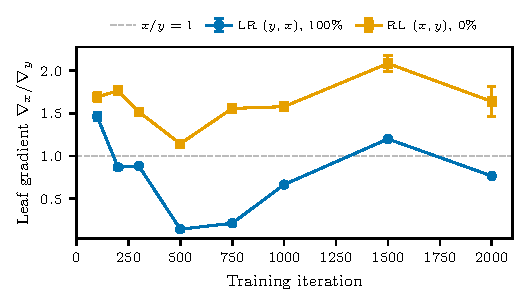
\includegraphics[width=\columnwidth]{fig_odrzywolek2026_gradient.pdf}
\Description{Leaf x/y gradient ratio trajectory for Eq.6 on a recovered vs an unrecovered target during search-phase training.}
\caption{Leaf-gradient ratio $\rho_{xy}(t) =
\|\nabla_{\theta_x} \mathcal{L}_t\| /
\|\nabla_{\theta_y} \mathcal{L}_t\|$ during Eq.\,6 search under
EML for a recovered LR target ($100\%$ recovery) and an
unrecovered RL target ($0\%$); 10-seed mean $\pm$ s.e.}
\label{fig:gradient}
\end{figure}

\begin{figure}[t]
\centering
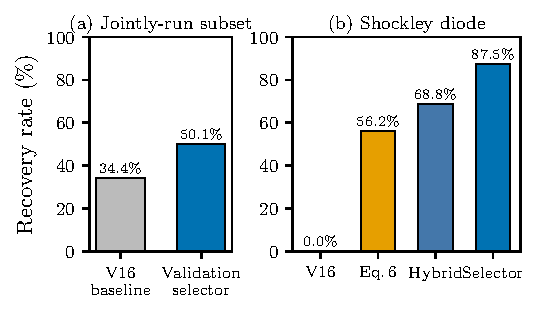
\includegraphics[width=\columnwidth]{fig_odrzywolek2026_selector.pdf}
\Description{Validation selector recovery compared to individual architectures on jointly-run synthetic targets and the Shockley diode.}
\caption{Held-out validation over a small architecture set
reduces architecture-specific recovery failures.  For each
target, the candidate with the lowest held-out RMSE is selected.
On the jointly-run subset, selection improves recovery over the
V16-only baseline; on a Shockley diode target, selection
combines complementary successes from Eq.\,6 and Hybrid.}
\label{fig:selector}
\end{figure}

\subsection{Validation-Selected Architecture and a Practical Target}
\label{sec:results-selection}

The reversals in Section~\ref{sec:results-interaction} suggest
a simple proof-of-concept mitigation.  Train a small candidate
set of architectures on the target, harden each candidate, and
select the expression with the lowest held-out RMSE.  The selector is evaluated on the subset of configurations where
V16 and at least one other architecture were both run: EML
LR\,$(y,x)$ (Eq.\,6 + V16), RML LR\,$(y,x)$ (Eq.\,6 + V16), and
SML LR\,$(y,x)$ (V16 + Hybrid).  Pooling
the $256$ common (seed, initialization) trials per
configuration, V16, the only single architecture present
on all three, recovers $264/768 = 34.4\%$.  The validation
selector recovers $385/768$ trials, or $50.1\%$
(Fig.~\ref{fig:selector}a).  Since this subset contains only
three configurations, the result should be read as evidence that
validation-based architecture selection is promising, not as a
complete benchmark.  On this subset, the validation selector
matches the per-target oracle because exact and non-recovery
runs separate by roughly five orders of magnitude in held-out
RMSE.  Re-running V16 with
Eq.\,6's initialization strategy on SML LR\,$(y,x)$ collapses
its rate from $84.4\%$ to $0/64$, so a deployable selector must
hold the per-architecture initialization set fixed.

As a representativeness check, we evaluate the Shockley diode
equation $I = I_0\,(\exp(qV/kT) - 1)$~\citep{Shockley1949pn},
a classic nonlinear electrical-engineering model with
signal-processing relevance.  The normalized Shockley diode
form, $\mathrm{eml}(x,e)$, is depth-1 in EML, so the diode
equation provides a useful target outside the synthetic target
family.
Under the same depth-3 protocol with $x \in [0, 5]$, Eq.\,6
recovers the target on $18/32$ seeds, Hybrid on $22/32$ seeds,
and V16 on $0/32$ seeds.  The selector chooses Eq.\,6 or Hybrid
in every recovered run and recovers $28/32$ seeds by covering
complementary successes across architectures
(Fig.~\ref{fig:selector}b).  V16's failure is representational
rather than optimizational.  V16 takes the variable~$x$ only at
leaves, so the root's left input must be either a constant or
the output of a depth-$\le 2$ V16 subtree, and exhaustive
enumeration of those outputs over $\{1, x, y\}$ contains no
expression equal to $x$.  In this experiment, a single fixed
V16 choice would yield zero recoveries.
